% XeLaTeX no Overleaf. 20 slides, roteiro de aproximadamente 12 minutos.
% Joey apresenta slides 1--10; Paulo apresenta 11--20.
\documentclass[aspectratio=169,11pt]{beamer}
\usepackage[T1]{fontenc}
\usepackage[utf8]{inputenc}
\usepackage[brazil]{babel}
\usepackage{lmodern,booktabs,amsmath,graphicx}
\definecolor{azul}{HTML}{172D3C}
\definecolor{verde}{HTML}{087F8C}
\setbeamercolor{normal text}{fg=azul,bg=white}
\setbeamercolor{frametitle}{fg=azul}
\setbeamercolor{structure}{fg=verde}
\setbeamercolor{block title}{fg=white,bg=verde}
\setbeamercolor{block body}{bg=verde!6}
\setbeamerfont{frametitle}{size=\Large,series=\bfseries}
\setbeamertemplate{navigation symbols}{}
\setbeamertemplate{itemize items}[circle]
\setbeamertemplate{footline}{\hspace{5mm}\scriptsize ENEM 2023 | Unifor\hfill\insertframenumber/\inserttotalframenumber\hspace{5mm}\vspace{3mm}}
\setbeamersize{text margin left=8mm,text margin right=8mm}
\graphicspath{{figuras/}}
\newcommand{\figura}[1]{\begin{center}\includegraphics[width=.96\linewidth,height=5.35cm,keepaspectratio]{#1}\end{center}}
\newcommand{\fonte}[1]{\par\vspace{1mm}{\tiny #1\par}}
\newcommand{\duas}[2]{\begin{columns}[T,onlytextwidth]\begin{column}{.48\textwidth}#1\end{column}\begin{column}{.48\textwidth}#2\end{column}\end{columns}}
\title{Comparação nacional de modelos\\ENEM 2023}
\author{Joey Alan de Freitas Solis \and Paulo Henrico}
\institute{Universidade de Fortaleza (Unifor)\\Professor Tulio}
\date{}

\begin{document}
\begin{frame}\titlepage\centering\textcolor{verde}{Previsão da nota de Ciências da Natureza a partir do perfil}\end{frame}
\begin{frame}{Problema e objetivo}
\begin{block}{Pergunta de pesquisa}Quanto o perfil socioeconômico, escolar e demográfico permite estimar a nota de Ciências da Natureza?\end{block}
\begin{itemize}\item Comparar dez regressores/configurações e a média de referência.
\item Medir erro e generalização entre participantes da mesma edição.
\item Investigar preparação, atributos, complexidade e desigualdade dos erros.
\end{itemize}
\fonte{Fonte dos dados: Inep, microdados do ENEM 2023. Estudo observacional, sem inferência causal.}
\end{frame}
\begin{frame}{Base nacional e participantes}
\duas{\begin{tabular}{lr}\toprule Base original & 3.933.955\\Sem alvo & 1.241.528\\Alvo observado & 2.692.427\\\midrule Desenvolvimento & 2.153.941\\Teste reservado & 538.486\\\bottomrule\end{tabular}}{\begin{itemize}\item 76 colunas na fonte; 40 entradas originais.
\item 16.547 notas zero mantidas.
\item Nota ausente não é zero nem é imputada.
\item Somente dados reais na modelagem nacional.\end{itemize}}
\fonte{Inep, 2023. ZIP e CSV originais preservados; 79 Parquets confrontados integralmente com o CSV normalizado.}
\end{frame}
\begin{frame}{Entradas e prevenção de vazamento}
\duas{\textbf{40 campos de perfil}\begin{itemize}\item Q005: moradores (numérico).
\item 15 campos demográficos/escolares, UF da prova e língua.
\item 24 questões categóricas: escolaridade, ocupação, renda, bens e acesso digital.\end{itemize}}{\textbf{Fora de X}\begin{itemize}\item NU\_INSCRICAO: somente controle.
\item NU\_NOTA\_CN: alvo.
\item Outras notas, presença, respostas e gabaritos excluídos.
\item Competências de redação não integradas.\end{itemize}}
\fonte{Lista completa: configs/ciencias\_natureza.toml. Registro das colunas: resultados/colunas.csv.}
\end{frame}
\begin{frame}{Preparação dos dados}
\begin{enumerate}\item Ingestão: espaços, tokens de ausência, tipos, ano, IDs e contagens.
\item Q005: mediana e padronização; indicador de ausência quando aplicável.
\item Categorias: ausência explícita e one-hot; desconhecimento preservado conforme o dicionário.
\item Transformações ajustadas somente no treino de cada dobra, dentro do pipeline.\end{enumerate}
\begin{block}{Representação original}235 dimensões nos ajustes registrados. Indicadores categóricos são binários; Q005 permanece numérica.\end{block}
\fonte{Código: cleaning.py, ingestion.py e preprocessing.py em src/enem\_base/.}
\end{frame}
\begin{frame}{Treinamento e validação cruzada}
\centering\begin{tabular}{lccc}\toprule Rodada & A (dobra 0) & B (dobra 1) & C (dobra 2)\\\midrule 1 & \textbf{Validação} & Treino & Treino\\2 & Treino & \textbf{Validação} & Treino\\3 & Treino & Treino & \textbf{Validação}\\\bottomrule\end{tabular}
\vspace{4mm}\begin{itemize}\item Desenvolvimento: 80\%; teste separado: 20\%; semente 42.
\item As mesmas três dobras e métricas para todos os modelos.
\item O teste não participa de seleção de atributos ou parâmetros.\end{itemize}
\fonte{IDs persistidos em dados/splits/. Dobras A/B/C: 717.981 / 717.980 / 717.980 participantes.}
\end{frame}
\begin{frame}{Todos os modelos obrigatórios foram comparados}
\small\begin{tabular}{p{3.1cm}p{10cm}}\toprule Modelo & Como produz a previsão\\\midrule
Linear / Ridge & Combinação linear; Ridge penaliza coeficientes grandes com L2.\\
Árvore & Regras sucessivas até regiões de nota média.\\
SVM linear & Função linear regularizada com perda insensível a epsilon.\\
KNN & Média ponderada dos 25 vizinhos euclidianos exatos.\\
Bagging / Pasting & Média de árvores em subamostras com / sem reposição.\\
Random Forest & Árvores e sorteio de atributos nas divisões.\\
Gradient Boosting & Árvores sequenciais para reduzir o erro.\\
Stacking & Combina previsões de linear e árvore com Ridge.\\
Média & Baseline: prevê a média aprendida no treino.\\\bottomrule\end{tabular}
\fonte{Três dobras completas por configuração inicial. Código: modeling.py; KNN exato: neighbors.py.}
\end{frame}
\begin{frame}{Stacking e o papel do Ridge}
\begin{block}{Bases}Regressão linear + árvore de decisão. Cada uma possui seu próprio pipeline.\end{block}
\begin{block}{Combinação sem vazamento}Três dobras internas geram previsões fora da dobra: cada participante é previsto por uma base que não treinou nele. Ridge aprende a combinar essas previsões.\end{block}
\[
\widehat{y}=b+w_1\widehat{y}_{\mathrm{linear}}+w_2\widehat{y}_{\mathrm{arvore}},\qquad
\min_{b,w}\ \sum_i(y_i-\widehat y_i)^2+\alpha\lVert w\rVert_2^2
\]
\fonte{Expressão estrutural: os coeficientes são aprendidos nos dados, não são constantes escolhidas manualmente.}
\end{frame}
\begin{frame}{Métricas e comparação justa}
\[
\mathrm{RMSE}=\sqrt{\frac{1}{n}\sum_i(y_i-\widehat y_i)^2}
\qquad
\mathrm{MAE}=\frac{1}{n}\sum_i|y_i-\widehat y_i|
\]
\begin{itemize}\item RMSE é o critério principal e penaliza mais os erros grandes.
\item MAE expressa erro absoluto médio; R\textsuperscript{2} compara ajuste à variabilidade das notas.
\item CV: média e desvio padrão populacional nas três dobras.
\item Teste: resultado único, separado da média de CV.
\item Tempos registrados; caches e cargas concorrentes limitam comparações de custo.\end{itemize}
\end{frame}
\begin{frame}{Comparação inicial do catálogo completo}
\figura{18_comparacao_completa.png}
\fonte{Trio global: Stacking, Ridge e linear. No recorte de sete algoritmos: Stacking, SVM e Random Forest.}
\end{frame}
\begin{frame}{Engenharia, seleção e aprofundamento}
\begin{itemize}\item Computadores por morador: contagem limitada de Q024 dividida por Q005 válida.
\item Acesso digital: presença de computador + internet (0 a 2).
\item Escolaridade dos responsáveis: máximo, quando ambas as respostas são conhecidas.
\item Seleção de 75\% dos atributos codificados por f\_regression, no treino.
\item Ablações: retirar questionário socioeconômico ou UF piorou o Ridge.
\item Ponderação de faixas raras: RMSE global piorou; não foi adotada.\end{itemize}
\fonte{Comparações nacionais nas mesmas dobras. Não se inferem efeitos causais de renda, escola ou localização. Código: variants.py.}
\end{frame}
\begin{frame}{PCA: compactação sem ganho preditivo}
\figura{05_pca.png}
\fonte{Desenvolvimento: limiar de 80\%; 45/235 componentes em cada ajuste de Ridge e árvore. O RMSE aumentou nos dois modelos; PCA não compõe a solução final.}
\end{frame}
\begin{frame}{Busca de hiperparâmetros no desenvolvimento}
\centering\begin{tabular}{lrr}\toprule Modelo & RMSE inicial & Menor RMSE da busca\\\midrule
Stacking & 76,174515932 & 76,174515900\\
Ridge & 76,483610 & 76,483572\\
Linear & 76,483799 & 76,483594\\
SVM linear & 76,576690 & 76,576690\\
Random Forest & 76,642872 & 76,642872\\\bottomrule\end{tabular}
\vspace{3mm}\begin{itemize}\item Cinco modelos; 12 configurações por modelo; 180 avaliações nas três dobras.
\item Melhorias pequenas não demonstram relevância prática ou significância.
\item Stacking final: Ridge combinador com alpha=1.000. Teste fora da busca.\end{itemize}
\fonte{GridSearchCV com dobras persistidas. Valores reais, arredondados para exibição. Fontes: tuning.py e final\_selection.py.}
\end{frame}
\begin{frame}{Curvas de aprendizado e generalização}
\figura{08_curvas_finais.png}
\fonte{Desenvolvimento: 10\%, 25\%, 50\%, 75\% e 100\% do treino, validação fixa; média e DP nas três dobras. Pequenos intervalos não comprovam desempenho em outro ano. Reuso compatível registrado.}
\end{frame}
\begin{frame}{Teste reservado: cinco receitas já congeladas}
\centering\begin{tabular}{lrrr}\toprule Modelo & RMSE & MAE & R\textsuperscript{2}\\\midrule
\textbf{Stacking} & \textbf{76,190} & \textbf{55,325} & \textbf{0,2497}\\
Linear de referência & 76,517 & 55,616 & 0,2433\\
SVM linear & 76,622 & 55,538 & 0,2412\\
Random Forest & 76,658 & 55,821 & 0,2405\\
Média & 87,959 & 66,285 & -0,000002\\\bottomrule\end{tabular}
\vspace{3mm}\begin{block}{Resultado final}538.486 participantes em comum. Stacking reduziu o RMSE em 13,38\% em relação à média.\end{block}
\fonte{O enunciado exige média, linear e solução final no teste. SVM e Random Forest são avaliações adicionais; os demais possuem CV completa.}
\end{frame}
\begin{frame}{Notas observadas versus previstas}
\figura{11_observado_previsto.png}
\fonte{Teste reservado completo. Diagonal: previsão perfeita. Concentração central: superestimação das notas baixas e subestimação das altas.}
\end{frame}
\begin{frame}{Os maiores erros aparecem nos extremos}
\duas{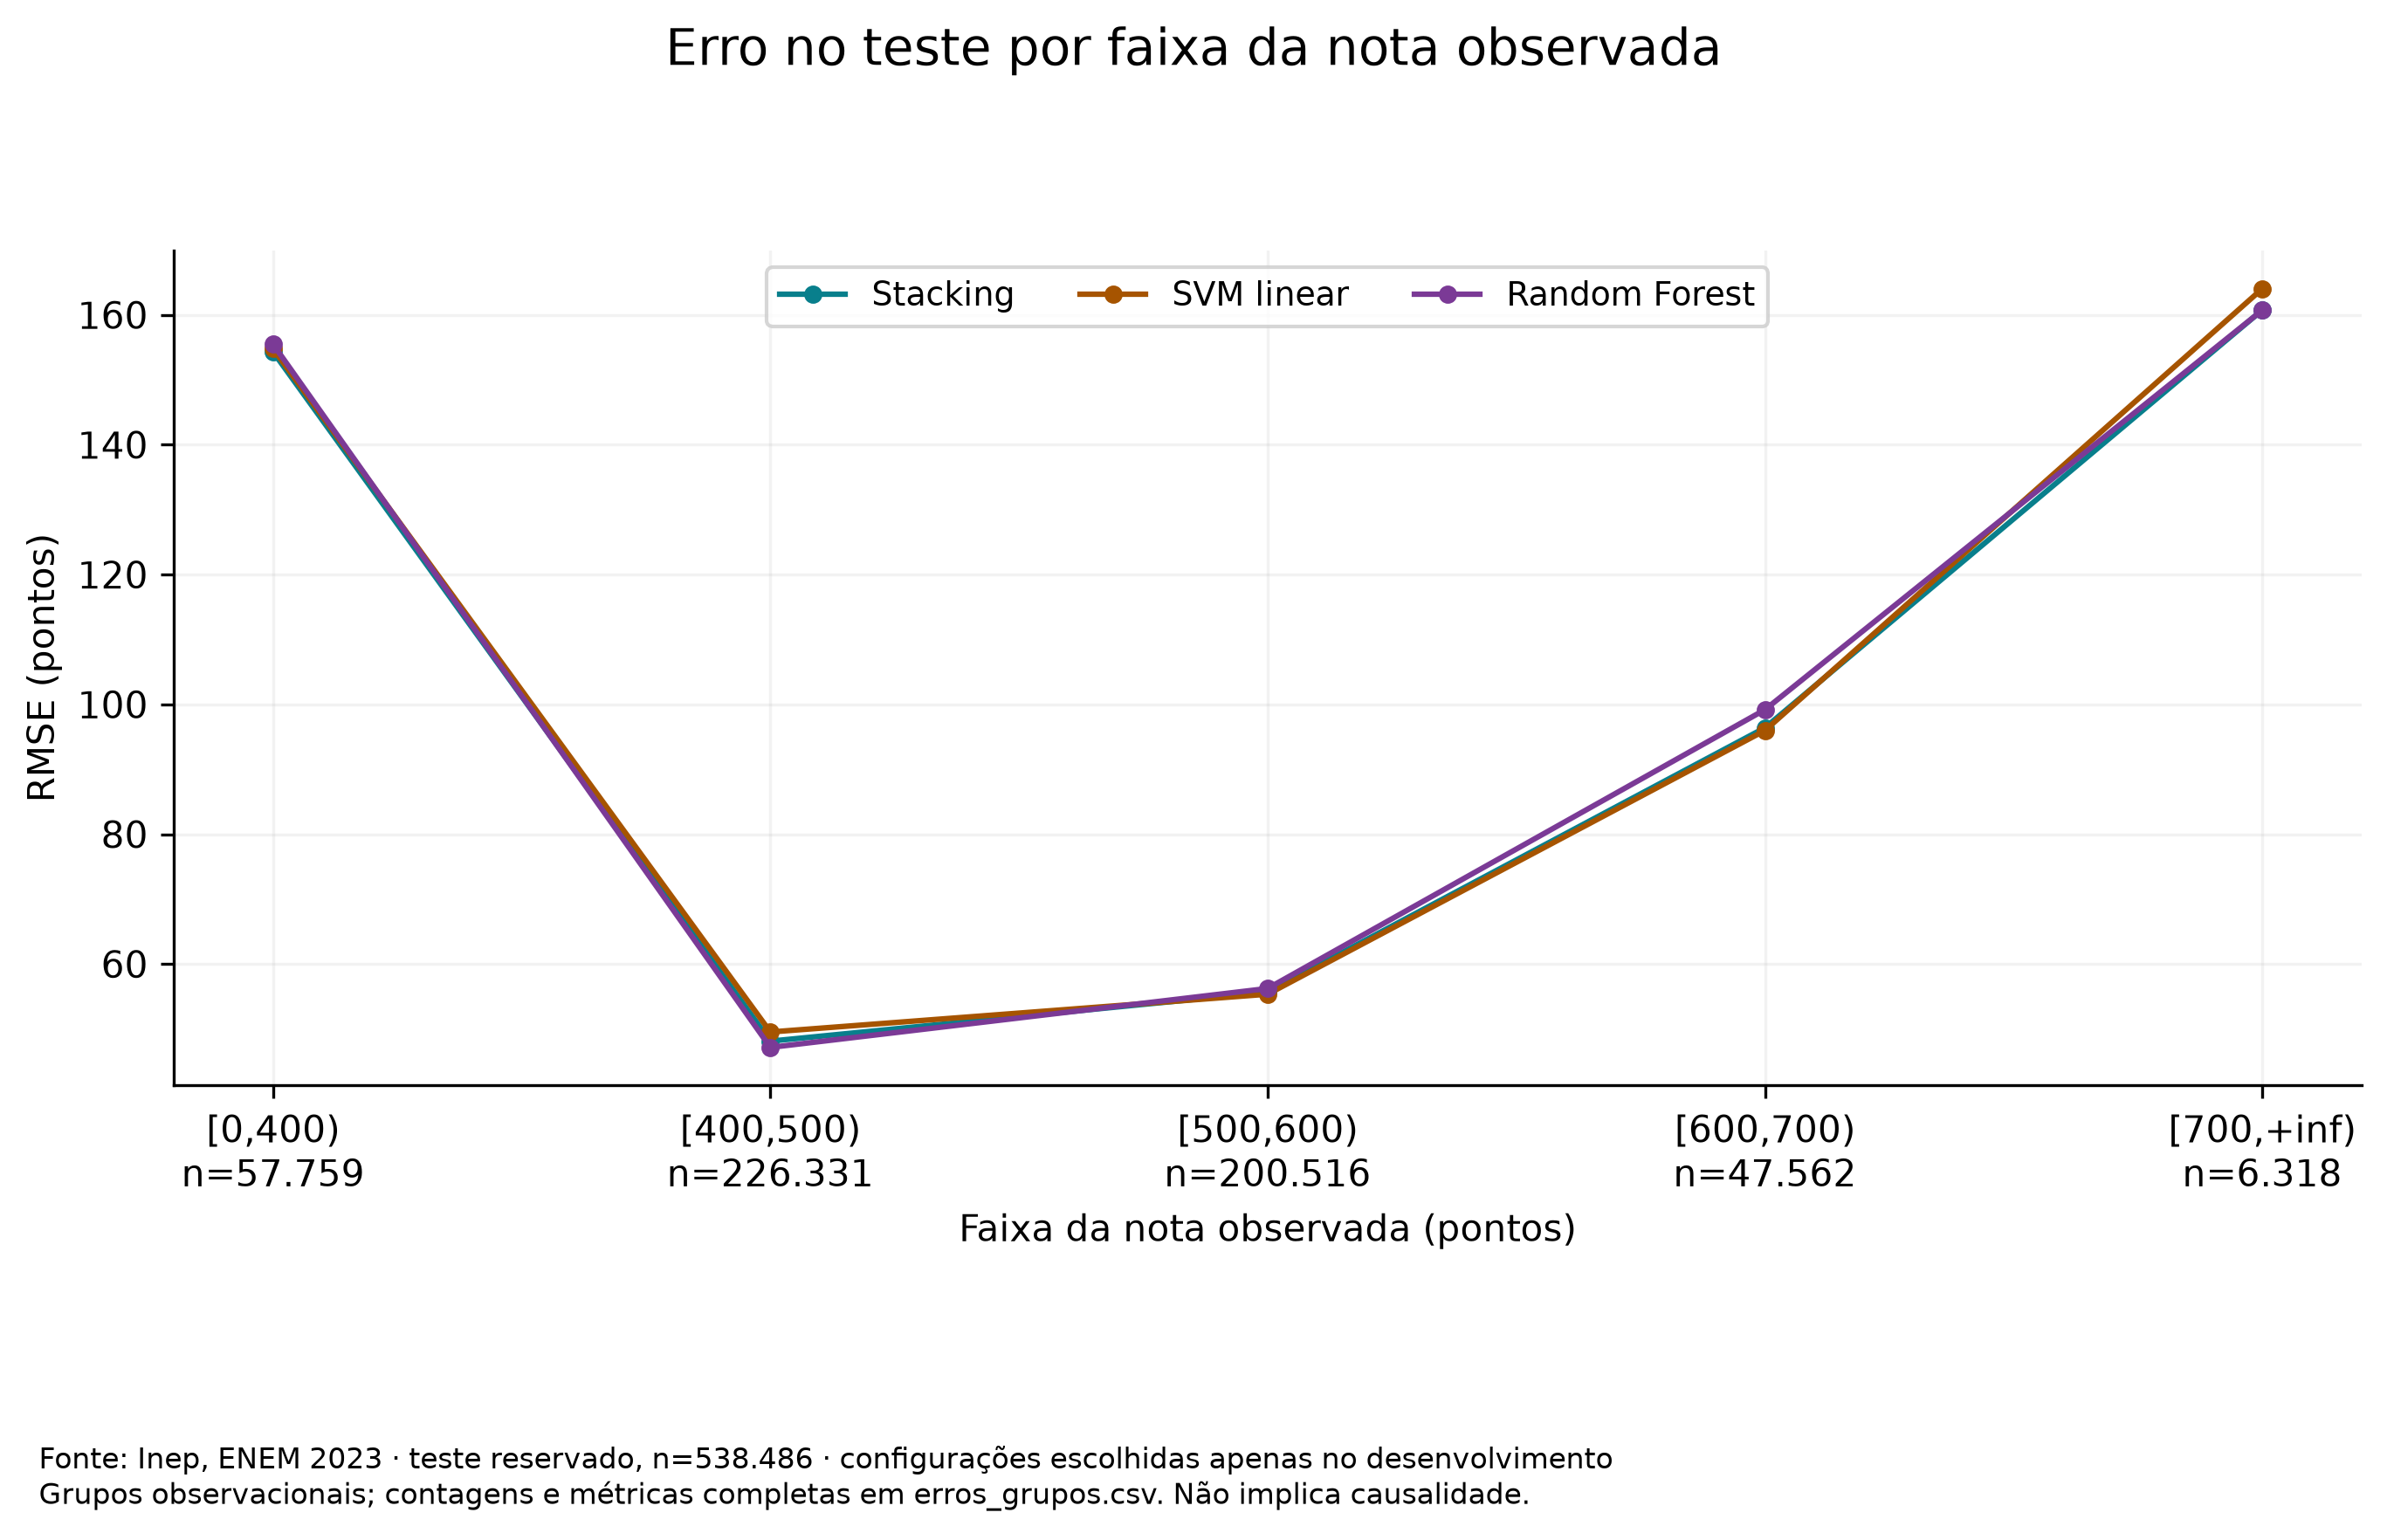
\includegraphics[width=\linewidth,height=5cm,keepaspectratio]{13_faixas.png}}{\begin{itemize}\item Abaixo de 400: RMSE 154,31; n=57.759.
\item Entre 400 e 500: RMSE 48,12; n=226.331.
\item A partir de 700: RMSE 160,74; n=6.318.
\item A métrica global não descreve bem todos os participantes.\end{itemize}}
\fonte{Teste, Stacking. Limites das faixas definidos antes da abertura do teste.}
\end{frame}
\begin{frame}{Erros por grupo e análise dos resíduos}
\duas{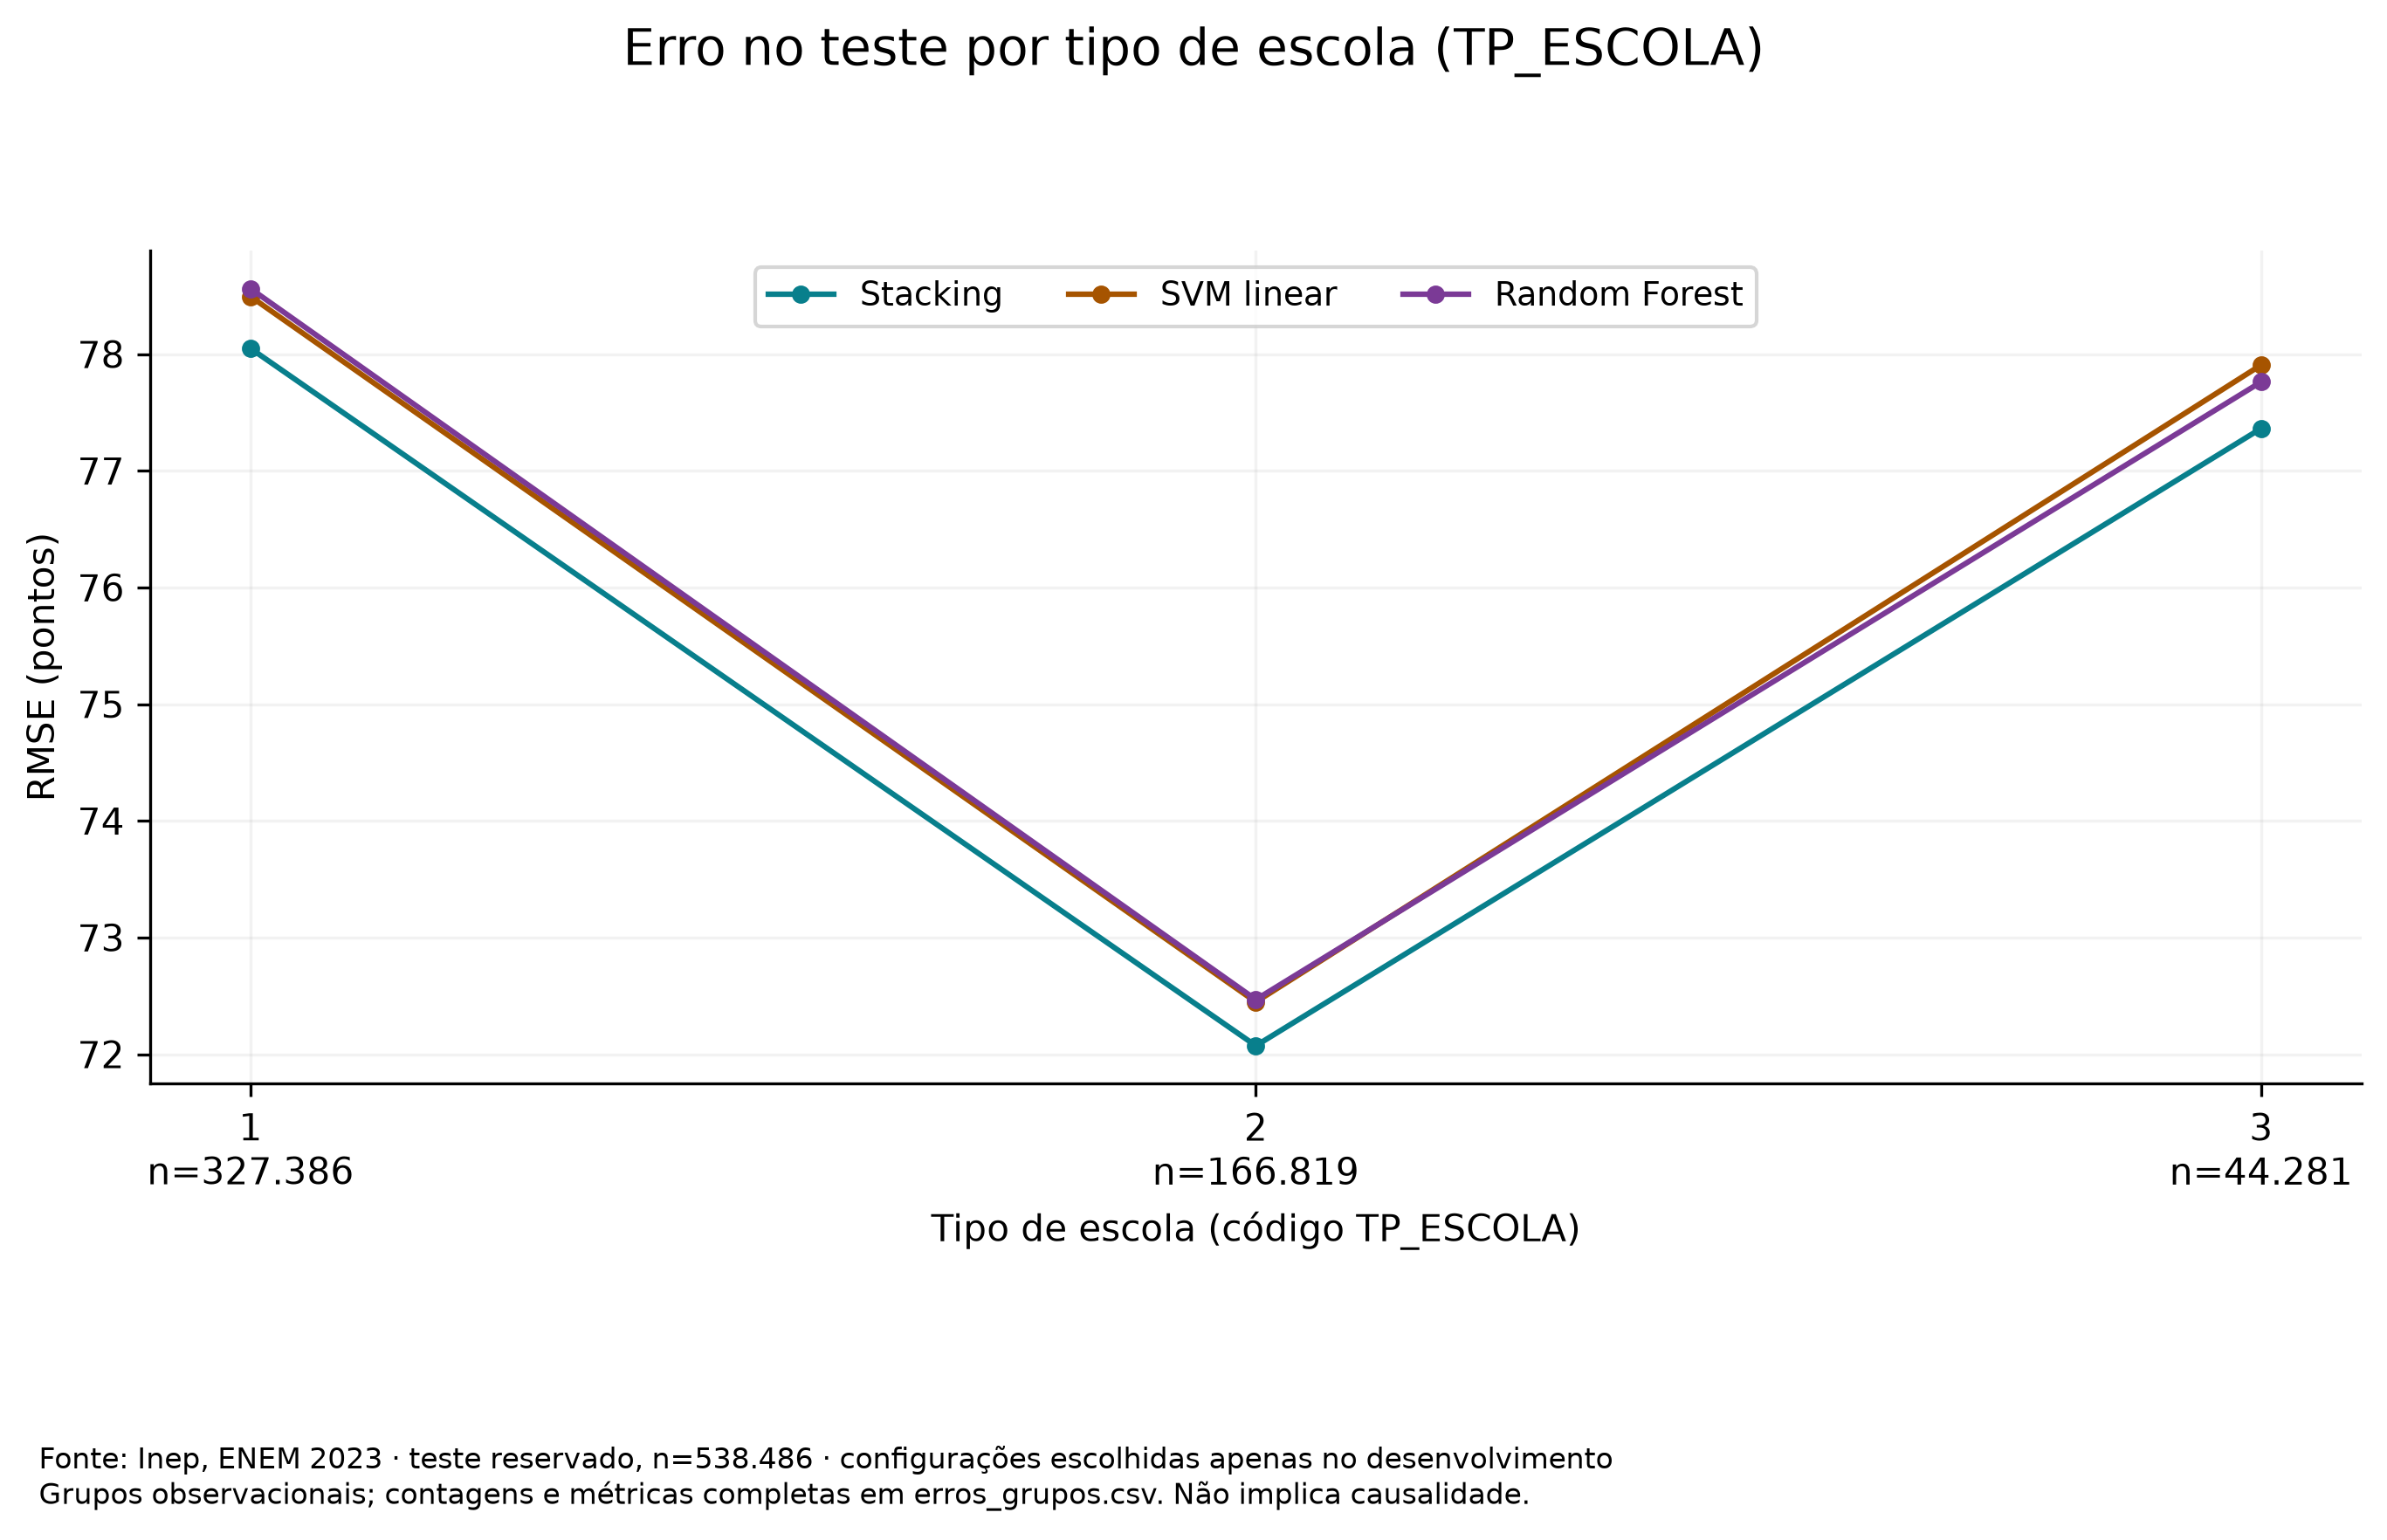
\includegraphics[width=\linewidth,height=5cm,keepaspectratio]{14_escola.png}}{\begin{itemize}\item TP\_ESCOLA=1: não informado; n=327.386.
\item Pública: n=166.819; privada: n=44.281.
\item Também há análises por renda, UF da prova e resíduos.
\item Comparação descritiva: grupos diferem em tamanho e composição.\end{itemize}}
\fonte{Fonte: Inep, ENEM 2023; teste reservado. UF da prova não é necessariamente UF de residência.}
\end{frame}
\begin{frame}{Reprodutibilidade e limites}
\begin{itemize}\item Originais, preparação, IDs de partição, código e resultados separados.
\item Configurações, métricas por dobra, tempos e hashes registrados.
\item Conferência independente: métricas recompostas das previsões já existentes.
\item Dados observacionais de uma edição; sem avaliação temporal ou causalidade.
\item Não houve teste de significância das pequenas diferenças entre modelos.
\item Previsões de perfil não determinam capacidade individual nem substituem avaliação.\end{itemize}
\fonte{Repositório: github.com/JoeyAlanS/trab2-aprendizado-de-maquina. Modelo e pipeline: src/enem\_base/.}
\end{frame}
\begin{frame}{Conclusões e próximos estudos}
\begin{block}{Conclusão}Todos os regressores obrigatórios foram comparados. Stacking teve o menor RMSE de desenvolvimento e apresentou RMSE 76,190 no teste reservado.\end{block}
\begin{itemize}\item O perfil ajuda a prever parte da variação, com limitações nos extremos.
\item Mais transformação ou complexidade não garantiu melhor desempenho.
\item Próximos estudos: outra edição, perdas para extremos e contexto externo.
\end{itemize}
\fonte{Referências: Inep (2023), microdados e dicionário; Pedregosa et al. (2011), Scikit-learn: Machine Learning in Python, JMLR 12, 2825--2830; Douze et al. (2024), The Faiss Library, arXiv:2401.08281. Referências completas no artigo.}
\end{frame}
\end{document}
